\documentclass[compress,xcolor=dvipsnames]{beamer}
%\documentclass[compress,xcolor=dvipsnames, handout]{beamer}


\usepackage[spanish]{babel}
\usepackage{graphicx}
\usepackage{grffile}

\usepackage{tikz}

\usepackage[export]{adjustbox}

\usepackage{pgfpages}


\usepackage{amsfonts,amssymb, amsmath}

\usepackage{MnSymbol}%
\usepackage{wasysym}%

\usepackage{latexsym}
\usepackage{enumerate}
\usepackage{xspace}
\usepackage{tabularx}
\usepackage{url}
\usepackage[utf8]{inputenc}
\usepackage{pgf, pgfnodes, pgfarrows}

\usefonttheme{serif}

\mode<presentation>{
\usetheme{lined}
}

\setbeamertemplate{navigation symbols}{}

\usepackage{times}
\usepackage[T1]{fontenc}

\title{Simetrías en lógicas de descripción}
\institute[Giovanni Rescia]{\large Giovanni Rescia}
\date{\small FaMAFyC\\~\\1 de Junio, 2017}

\newtheorem{teorema}{Teorema}
\newtheorem{proposicion}{Proposición}
\theoremstyle{definition}
\newtheorem{definicion}{Definición}
\newtheorem{notacion}{Notación}
\newtheorem{corolario}{Corolario}

\graphicspath{ {/Users/giovannirescia/coding/tesis/doc/gfx/presentacion} } 


\begin{document}

\beamerdefaultoverlayspecification{}

\newcommand{\tup}[1]{\langle #1 \rangle}
\newcommand{\cset}[1]{\{ #1 \}}
\newcommand{\csetsc}[2]{\{#1 \mid #2\}}
\newcommand{\PROP}{\textsf{PROP}\xspace}
\newcommand{\REL}{\textsf{REL}\xspace}
\newcommand{\cA}{\mathcal{A}\xspace}
\newcommand{\cD}{\mathcal{D}\xspace}
\newcommand{\cI}{\mathcal{I}\xspace}
\newcommand{\cM}{\mathcal{M}\xspace}
\newcommand{\cN}{\mathcal{N}\xspace}
\newcommand{\cS}{\mathcal{S}\xspace}
\newcommand{\Diam}[1]{\tup{#1}}
\newcommand{\st}{\textsf{ST}\xspace}
\newcommand{\flechita}{\leftrightsquigarrow}
\newcommand{\diam}[1]{\langle #1 \rangle}
\newcommand{\model}{\mathcal{M}}

\begin{frame}[plain]
\titlepage{}
\end{frame}
%% Introducción de la introducción
\begin{frame}
\frametitle{Introducción}
\begin{itemize}
\item Introducción: intuición, conceptos básicos, qué se hizo en esta tesis
\item Marco teórico del trabajo
\item Detalles de implementación
\item Evaluación empírica y análisis de resultados obtenidos
\end{itemize}
\end{frame}

%% Introducción
\begin{frame}
	\frametitle{Introducción}
  \begin{block}{}
    \begin{columns}[onlytextwidth,T]
      \column{\dimexpr\linewidth-30mm-5mm}
		\begin{itemize}[<+->]
			\item Concepto principal: simetría
			\item Contexto: RA / LF
			\item Ejemplo: SAT
			\item Simetría: permutación de variables que mantiene modelos
		\end{itemize}
		\onslide<+->
      	\column{30mm}
      	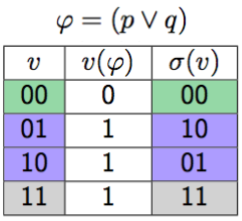
\includegraphics[width=30mm]{gfx/sym_ex}
    \end{columns}
  \end{block}
\end{frame}

%% Introducción
\begin{frame}
	\frametitle{Introducción}
  \begin{block}{}
    \begin{columns}[onlytextwidth,T]
      \column{\dimexpr\linewidth-20mm-2mm}
		\begin{itemize}
			\item Concepto principal: simetría
			\item Contexto: RA / LF
			\item Ejemplo: SAT
			\item Simetría: permutación de variables que mantiene modelos
		\end{itemize}
		\begin{itemize}[<+->]
					\item En particular aquí: \textcolor{blue}{lógicas de descripción} (DL)
			\item Estudio: detección y uso de simetrías
			\begin{itemize}[<.->]
				\item Aquí: solo detección
			\end{itemize}
			\item Enfoque:
				\begin{itemize}[<+->]
					\item Todo de cero
					\item \alert<+->{Aprovechando nexos y estudios previos en lógica modal}
				\end{itemize}
		\end{itemize}
      	\column{30mm}
      	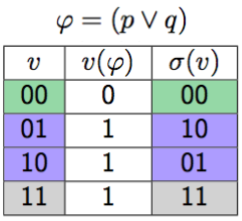
\includegraphics[width=30mm]{gfx/sym_ex}
    \end{columns}
  \end{block}
\end{frame}

\begin{frame}
\frametitle{Lógicas de descripción}
\begin{itemize}[<+->]
	\item Un subconjunto decidible de LPO
	\item DLs con diferentes expresividades
	\item Utilizadas para la representación de conocimiento
	\item Una base de conocimiento es una tupla <TBox, ABox> y define una ontología
		\begin{itemize}[<+->]
			\item Una ontología puede pensarse como conocimiento jerárquico, como una generalización de una taxonomía
		\end{itemize}
	\item Expresamos estas ontologías en una computadora a través de OWL
	\begin{itemize}[<+->]
			\item OWL es un formato estandar para expresar ontologías
		\end{itemize}
\end{itemize}
\end{frame}

\begin{frame}
	\frametitle{Lógicas de descripción (cont.)}
	
	\begin{itemize}[<+->]
		\item Un lenguaje para definiciones de conceptos
		\begin{itemize}[<+->]
			\item TBox
			\begin{itemize}[<+->]
				\item $Persona$ $\equiv$ $Mujer$ $\sqcup$ $Hombre$
				\item \textit{Padre} $\equiv$ $Persona$ $\sqcap$ $\exists$ $tieneHijo.Persona$
			\end{itemize}
		\end{itemize}
		\item Un lenguaje para aserciones
			\begin{itemize}[<+->]
				\item ABox
				\begin{itemize}[<+->]
					\item $tieneCapital(Italia, Roma)$
					\item \textit{Músico(Mozart)}
				\end{itemize}
			\end{itemize}
		\item Modelos relacionales
	\end{itemize}
\end{frame}

\begin{frame}
	\frametitle{Lógicas modales}
	\begin{itemize}[<+->]
		\item Desarrollada en los 60
		\item Extiende a la lógica proposicional, incluyendo modalidades
		\begin{itemize}[<+->]
			 \item $[m_{i}] p  \lor \langle m_{j} \rangle q$
		\end{itemize}
	\item Utilizada para model checking
	\item Un ejemplo particular de lógica modal: Lógica temporal
	\item Modelos relacionales (como en DL)
	\end{itemize}
	\onslide<+->
	\begin{center}
		\begin{tabular}{ c |  c }
			ML & DL \\ \hline
			$p_{i}$ & $C_{i}$, y $C_{i}$ es un concepto atómico \\ \hline
			$\neg \varphi$ & $\neg C$, y $C$ es un concepto		\\ \hline
			$\varphi \lor \Psi $ &	$C_{j}\sqcup C_{i}$, con $Cj,\,C_{i}$ conceptos		\\ \hline
			$\langle R \rangle \varphi$  &   $\exists R.C_{j}$, y $R$ es un rol atómico y $C_{j}$ es un concepto		\\ \hline
		\end{tabular}
	\end{center}
	
\end{frame}


\begin{frame}[<-+>]
	\frametitle{De OWL a ML}
	Ya vimos que existe un nexo sintáctico y semántico entre DL y ML
	\pause
	
	
	\begin{tabular}{r  c  l}
	& & \\
	$\Psi(\mathcal{R}\,someValuesFrom\,\mathcal{C})$ & $\doteq$ & $\langle\mathcal{R}\rangle\Psi(\mathcal{C})$ \\
	$\Psi(complementOf(\mathcal{C}))$ & $\doteq$ & \textbf{\large{}$\neg\Psi(\mathcal{C})$} \\
	$\Psi(SubClassOf(\mathcal{C}_{1}\,\mathcal{C}_{2}))$ & $\doteq$ & $A(\Psi(\mathcal{C}_{1})\implies\Psi(\mathcal{C}_{2}))$ \\
	$\Psi(EquivalentClasses(\mathcal{C}_{1}\equiv\mathcal{C}))$ & $\doteq$ & $\Psi(\mathcal{C}_{1}\sqsubseteq\mathcal{C}_{2})\land\Psi(\mathcal{C}_{2}\sqsubseteq\mathcal{C}_{1})$ \\
	$\Psi(unionOf(\mathcal{C}_{1}\,\mathcal{C}_{2}))$ & $\doteq$ & $\Psi(\mathcal{C}_{1})\lor\Psi(\mathcal{C}_{2})$ \\
\end{tabular}
\end{frame}

\begin{frame}
	\frametitle{Simetrías}
		\begin{center}
		\begin{tikzpicture}
			\node (img1) {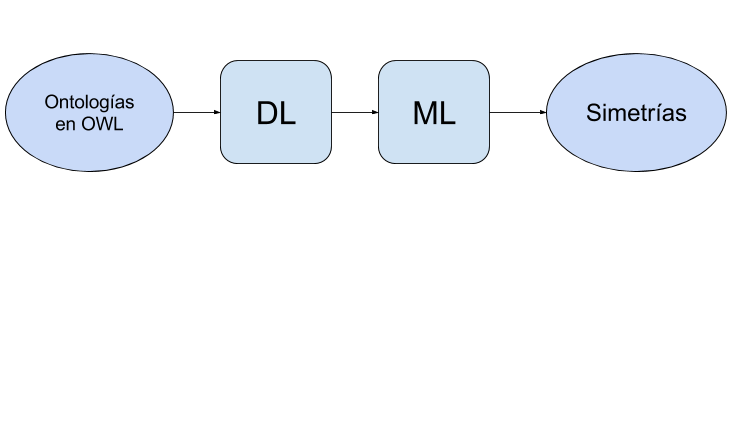
\includegraphics[scale=0.3]{gfx/bp2.png}};
			\pause
			\node (img2) {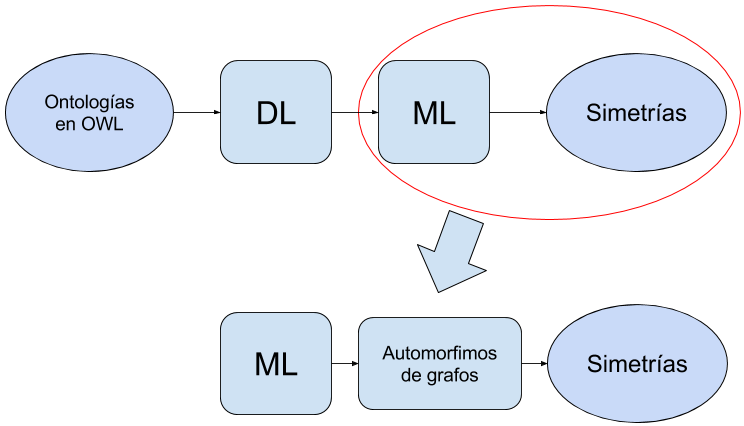
\includegraphics[scale=0.3]{gfx/bp2.1.png}};
		\end{tikzpicture}
	\end{center}
\end{frame}

\begin{frame}
	\frametitle{Pipeline de procesamiento}
		\begin{center}
		\begin{tikzpicture}
			\node (img1) {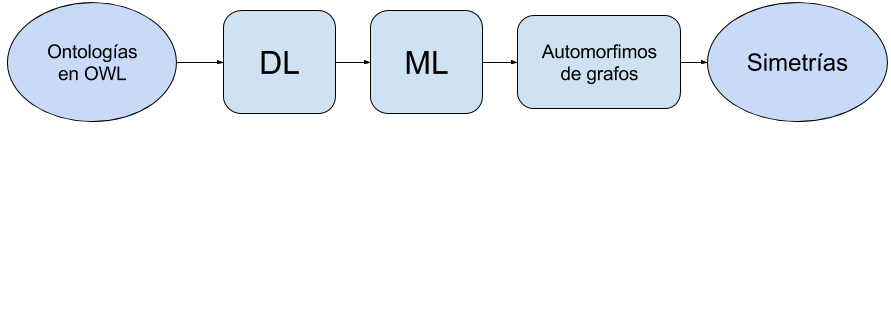
\includegraphics[scale=0.3]{gfx/bp3.png}};
			\pause
			\node (img2) {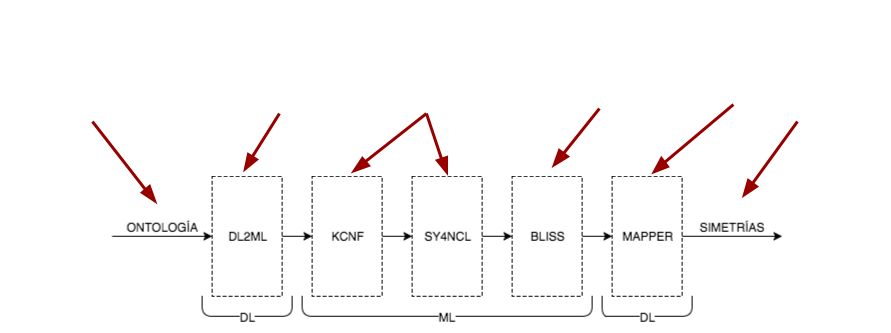
\includegraphics[scale=0.3]{gfx/bp3.1.png}};
		\end{tikzpicture}
	\end{center}
\end{frame}

\begin{frame}
\frametitle{Ejemplo de base de conocimiento}
TBox=
	\begin{center}
		\begin{tabular}{rll}
			$gato$ & $\sqsubseteq$ & \textit{mamífero} \\
			$perro$ & $\sqsubseteq$ &\textit{mamífero} \\
			$caballo$ & $\sqsubseteq$ & \textit{mamífero} \\
			$gatito$ & $\equiv$ & $gato\sqcap\exists $ \textit{críaDe.gato}\\
			$cachorro$ & $\equiv$ & $perro\sqcap\exists $ \textit{críaDe.perro}\\
			$potrillo$ & $\equiv$ & $caballo\sqcap\exists $ \textit{críaDe.caballo}\\
			$gato$ & $\sqsubseteq$ & $mam\acute{\imath}fero\sqcap\exists $\textit{cuadrúpedo.mamífero}\\
			$perro$ & $\sqsubseteq$ & $mam\acute{\imath}fero\sqcap\exists $\textit{cuadrúpedo.mamífero}\\
			$caballo$ & $\sqsubseteq$ & $mam\acute{\imath}fero\sqcap\exists $\textit{cuadrúpedo.mamífero}\\
		\end{tabular}
	\end{center}
\end{frame}

\begin{frame}
	\frametitle{DL2ML}
	\begin{itemize}[<+->]
		\item Toma la ontología en OWL y devuelve la fórmula modal 
		\item Implementado para esta tesis
		\item Programado en Scala
		\begin{itemize}[<+->]
			\item Con la API de Scowl (wrapper de la API de OWL)
		\end{itemize}
		\item Trabaja solo sobre la TBox de la ontología
	\end{itemize}
	\onslide<+->
	\begin{center}
    	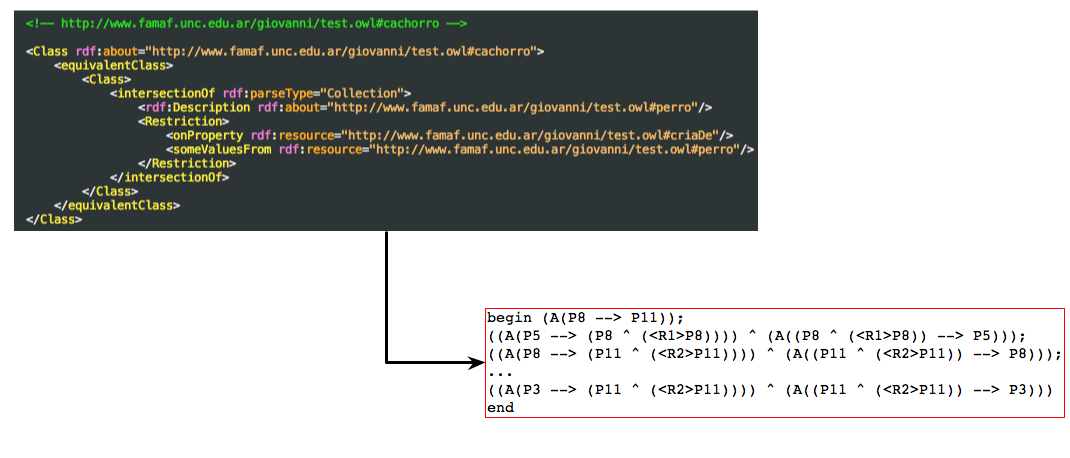
\includegraphics[scale=0.305, left]{gfx/dl2ml}
	\end{center}

\end{frame}

\begin{frame}
	\frametitle{KCNF}
	\begin{itemize}[<+->]
		\item Retorna la CNF de una fórmula modal
		\item Desarrollado en Haskell
		\item Adaptado para este proyecto
	\end{itemize}
	\onslide<+->
	\begin{center}
    	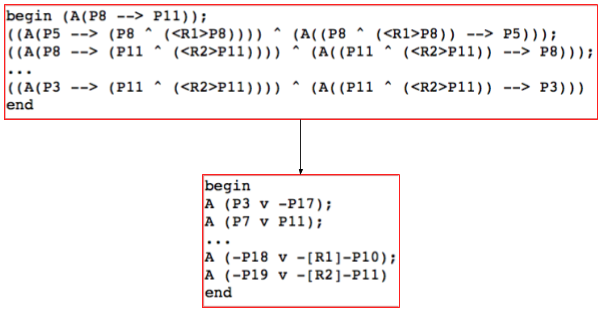
\includegraphics[scale=0.305]{gfx/kcnf}
	\end{center}
\end{frame}


\begin{frame}
	\frametitle{SY4NCL}
	\begin{itemize}[<+->]
		\item Crea el grafo de una fórmula en CNF
		\item Desarrollado en Haskell
		\item Adaptado para este proyecto
	\end{itemize}
		\onslide<+->
	\begin{center}
    	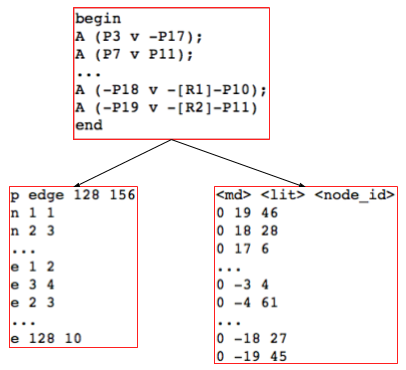
\includegraphics[scale=0.3225]{gfx/sy4ncl}
	\end{center}
\end{frame}

\begin{frame}
	\frametitle{BLISS}
	\begin{itemize}[<+->]
		\item Desarrollado en C++
		\item Automorfismos en grafos
	\end{itemize}
		\onslide<+->
	\begin{center}
    	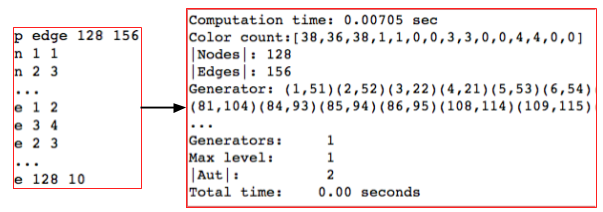
\includegraphics[scale=0.3525]{gfx/bliss}
	\end{center}
\end{frame}

\begin{frame}
	\frametitle{MAPPER}
	\begin{itemize}[<+->]
		\item Python, adaptado
		\item Nodos del grafo -> variables proposicionales -> conceptos de la ontología
	\end{itemize}
		\onslide<+->
	\begin{center}
    	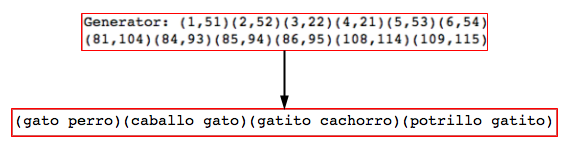
\includegraphics[scale=0.5525]{gfx/mapper}
	\end{center}
\end{frame}

\begin{frame}
	\frametitle{Set de datos}
	\begin{itemize}[<+->]
		\item +20 Ontologías obtenidas en la web
		\item La mayoría utilizadas por razonadores
		\item Diferentes expresividades
		\item Algunas muy conocidas	
		\begin{itemize}[<+->]
			\item Go: vocabulario de términos sobre material bioquímico
			\item NCIT: vocabulario para la atención clínica, información pública, etc.
			\item Uberon: ontología de anatomía para representar partes del cuerpo
		\end{itemize}
	\end{itemize}
\end{frame}

\begin{frame}
	\frametitle{Resultados}
	\begin{itemize}[<+->]
	\item Go
		\begin{itemize}[<.->]
		\item Tamaño de la TBox: 104783
		\item Tamaño del grafo: Nodos: 432315, Aristas: 528394
		\item Generadores detectados: 8496
		\item Tiempo para la detección de automorfismos: 57.93 seg.
		\end{itemize}
	\item NCIT
		\begin{itemize}[<.->]
		\item Tamaño de la TBox: 46940
		\item Tamaño del grafo: Nodos: 164267, Aristas: 183694
		\item Generadores detectados: 10218
		\item Tiempo para la detección de automorfismos: 37.24 seg.
		\end{itemize}
	\item Uberon
		\begin{itemize}[<.->]
		\item Tamaño de la TBox: 25683
		\item Tamaño del grafo: Nodos: 107903, Aristas: 135288
		\item Generadores detectados: 818
		\item Tiempo para la detección de automorfismos: 6.18 seg.
		\end{itemize}
	\end{itemize}
\end{frame}

\begin{frame}
	\frametitle{Análisis}
	\begin{itemize}
		\item Simetrías en todas las ontologías utilizadas
		\item Tiempo despreciable
		\item Memoria despreciable
	\end{itemize}
\end{frame}

\begin{frame}
	\frametitle{Trabajo futuro}
	\begin{itemize}
		\item Solo trabajamos con la TBox de cada ontología
			\begin{itemize}
				\item Extender $\Psi$ para que traduzca la ABox también
			\end{itemize}
	\item Implementar las simetrías en los razonadores para en cuánto mejora el rendimiento de los mismos
	\end{itemize}
\end{frame}

\begin{frame}
	\frametitle{Outro}
		\begin{center}
			\large	Preguntas?
		\end{center}
	\end{frame}
\end{document}
